\documentclass[11pt,a4paper,twoside,%
BCOR12mm,DIV14,%
headsepline,
cleardoubleempty,chapterprefix,parskip,%
liststotoc,bibtotoc]{scrbook}

% \usepackage[english, ngerman]{babel}
\usepackage[english]{babel}
\usepackage[utf8]{inputenc}
\usepackage[T1]{fontenc}
\usepackage{mathptmx}
\usepackage[scaled=0.92]{helvet}
\usepackage{courier}
\usepackage{mathtools}
 \usepackage{float}
\makeatletter
\def\displaymath{\typeout{*** Do not use DISPLAYMATH. Use \[...\] instead ***}}
\def\eqnarray{\typeout{*** Do not use EQNARRAY(*). Use align(*)-environment instead ***}}
\makeatother
\usepackage{amsfonts}
\usepackage{amstext}
\usepackage{subfigure}
\usepackage{color}
\usepackage{graphicx}

\graphicspath{ {fig/} }
\usepackage{ifpdf}
% \usepackage{makeidx}
% \usepackage{nomencl}
\usepackage{setspace}

% first include the hyperref package, then the cite package
\usepackage[plainpages=false,pdfpagelabels]{hyperref}
\usepackage{cite}

\setcounter{secnumdepth}{3}
\setcounter{tocdepth}{3}

% 
% Meta informationen to the thesis
% 

% Title of the Master Thesis
\newcommand{\thesistitle}{A Real-time Streaming Protocol for Large-scale Peer-to-Peer Networks}

% Name of the student
\newcommand{\thesisauthor}{Christopher Michael Probst}

% Place of Birth of the 
\newcommand{\thesisauthorbirthplace}{Solingen}

% Betreuer des Studenten
% Bei mehreren Betreuern bitte mit \\ trennen
\newcommand{\thesissupervisor}{Andreas Disterhöft M.Sc.}

% Schlagw\"orter zur Abschlussarbeit (optional)
\newcommand{\thesiskeywords}{}

% Abgabedatum: Tag
\newcommand{\thesissubmissionday}{1}

% Abgabedatum: Monat (als Wort)
\newcommand{\thesissubmissionmonth}{November}

% Abgabedatum: Jahr
\newcommand{\thesissubmissionyear}{2014}



\usepackage{lscape}
\usepackage{tabularx}



\ifpdf
    \definecolor{brown}{cmyk}{0, 0.81, 1, 0.60}
    \hypersetup{%
      pdftitle={\thesistitle{}},
      pdfsubject={Bachelor Thesis},
      pdfauthor={\thesisauthor{}},
      pdfkeywords={\thesiskeywords{}},
      colorlinks=false, urlcolor=blue, citecolor=brown,
      bookmarksnumbered=true,
    }
\else   
\fi

\listfiles

\begin{document}
\onehalfspacing

\frontmatter

\pdfbookmark[0]{Title Page}{tit}

\include{bachelor-titlepage}

\cleardoublepage

%!TEX root = bachelor.tex

\pdfbookmark[0]{Abstract}{abstract}
\begin{center} 
\huge Abstract
\end{center}


This thesis concentrates on implementing and evaluating different distribution algorithms for generic data transfers in large-scale \emph{Peer-to-Peer} networks, especially for incremental transfers, which yields the possibillity for video streaming. The main focus is on $1:n$ scenarios, where only one peer has a complete data set and $n$ peers try to distribute this data set among themselves as fast as possible.

The main problem is the choice of the best distribution algorithm, which should be able to use most of the available network bandwidth of all participating peers. In a traditional client\,/\,server system, the server uploads the data set to all clients sequentially, which means that only the server upload bandwidth is used but none of the client upload bandwidths.

Peer-to-Peer networks in combination with efficient distribution algorithms can help to solve this particular problem. These algorithms are always based on the same technique, where all participating peers download specific chunks from the peer, which has the complete data set and upload these chunks to other peers as well. This way, the peers help to distribute the data set using their own upload bandwidth. The difficulty is the choice of the specific chunks the peers download and the tuning of parameters like chunk count and chunk size.

In the course of this thesis, three distribution models are developed and evaluated. The main goal is to find a distribution model, that can distribute a data set evenly among all peers within $2\:*\:T_0$ seconds, where $T_0$ is the time to transfer the data set from one peer to another. Only the \emph{Chunked-Swarm} model was able to keep this limit. Therefore, the majority of the evaluation is dedicated to this model.

The evaluation of the Chunked-Swarm model shows, that this model works fine in general, but has some performance issues under high pressure. These issues are mostly based on the choice of the programming language, which is Java, and the pull based approach, which causes an exponentially growing amount of overhead. 

\cleardoublepage

%!TEX root = bachelor.tex

\pdfbookmark[0]{Danksagung}{ack}
\begin{center} 


\huge Acknowledgments

\end{center}

First I would like to thank Jun.-Prof. Dr.-Ing. Kalman Graffi and my supervisor Andreas Disterhöft for their professional and comprehensive support. Without them, this thesis would not be in its present form. I am particularly grateful for Andreas Disterhöft's assistance during the evaluation.

Furthermore, I would like to express my gratitude to my parents, who always supported me and made all of this possible, and my sister, who helped me in difficult situations to stay focused.

I also thank Matthias Hesse, who helped me out in several cases by taking off obligations of mine, which would have prevented me to work on the thesis.



\cleardoublepage

\pdfbookmark[0]{\contentsname}{content}
\tableofcontents

\listoffigures

\listoftables

\mainmatter

\cleardoublepage

%%%%%%%%%%%%%%%%%%%%%%%%%%%%%%%%%%%%%%%%%%%%%%
%%    Beginning of the main document        %%
%%                                          %%
%%    Include your tex-files with \input{}  %%
%%%%%%%%%%%%%%%%%%%%%%%%%%%%%%%%%%%%%%%%%%%%%%

\chapter{Introduction}
\section{Problem and Motivation}
Traditional networks are mostly based on the client/server model where the server only responds to client requests and the clients do not know each other. Depending on the application the server has to provide enough bandwidth to serve the clients fast enough.

In case of real-time video streaming, a server has to guarantee, that new clients will not influence the performance of running video streams of the remaining clients, which are already connected to the server. The consequence of that is, that a video streaming server can fundamentally only serve a certain number of clients, which are able to watch the video stream fluently, so this approach has scalability issues.

To improve this unbalance the clients could use their own upload capacity to help the server distributing a given data set. In this case the network is called a P2P network, where every participant is called a peer. If all peers have enough upload bandwidth, it is possible to create a P2P network, which is able to distribute a given data set evenly among all peers in a fixed time relative to the number of participating peers.

\section{Objective}
This thesis concentrates on implementing a P2P network, which is able to distribute a given data set among any number of clients and never exceeds $2 \cdot T$ where $T$ is the time needed for a single transfer between the server and a client measured in seconds.

To reach this goal different distribution algorithms are implemented and evaluated to compare advantages and disadvantages. The resulting software is able to measure those algorithms in terms of efficiency, overhead and performance.

The solution is generic and can be used for any kind of data set transfers like video streaming or large file transfers.

\section{Structure}
The thesis starts with evaluating existing concepts in chapter \ref{ch:relatedwork} and comparing them with the concepts, which are proposed and theoretically discussed in chapter \ref{ch:theory}. Then the architecture of the software is explained in chapter \ref{ch:arch}. The framework and application modules are presented in chapter \ref{ch:framework} and \ref{ch:app} respectively. The evaluation of the software follows in chapter \ref{ch:eval}.
\cleardoublepage
\chapter{Related work}
\label{relatedwork}
\cleardoublepage
\chapter{Theory}
\label{ch:theory}

\section{Model: Sequential}
\label{sec:sequentialmodel}
In the sequential (client/server) model, as shown in figure \ref{fig:sequentialmodel}, every client is only connected to the server. The server transfers data sets to all clients in parallel and thus all clients share the upload bandwidth of the server. This concept does not scale well, because every new client connecting to the system slows down every other client connected to the same server. 

\begin{figure}[H]
\centering
\includegraphics[width=6cm]{sequentialmodel}
\caption{Sequential distribution}
\label{fig:sequentialmodel}
\end{figure}

If $b$ is the bandwidth of the server in bytes/second, $n$ the number of clients connected to the server and $s$ the size of the whole data set, then $T= n \cdot T_0$ is the time in seconds it would take to transfer the data set to all clients, where $T_0=\frac{s}{b}$ is the time in seconds for a single tranfser from the server to a client. This formula assumes, that the download bandwidth of each client is bigger than the shared upload bandwidth. Without adding servers or using the upload bandwidth of the clients this linear relationship cannot be removed. This traditional model is implemented in the Sequential algorithm, which can be found in section \ref{subsubsec:seqlog}.

From the very first beginning it was clear, that this model is not able to keep the limit of $2 \cdot T_0$ seconds but it is implemented to show the immense difference. The next section \ref{sec:logarithmicmodel} presents a much better model.

\pagebreak
\section{Model: Logarithmic}
\label{sec:logarithmicmodel}
If a P2P network is used instead of a client/server model, where every participant is called a peer and has a connection to one or more other peers in the network. The number of connections depends on the used topology. In this thesis only the mesh topology is of importance, as shown in figure \ref{fig:peermesh}, where every peer is connected to every other peer in the network.

\begin{figure}[H]
\centering
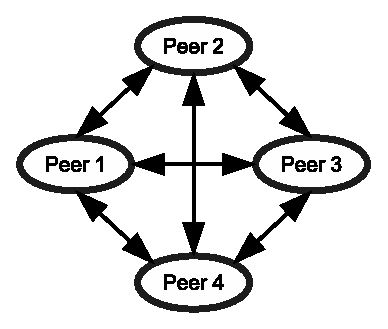
\includegraphics[width=6cm]{peermesh}
\caption{Peer mesh}
\label{fig:peermesh}
\end{figure}

In the logarithmic model every peer can do both uploading and downloading data sets. The only restriction is, that it can only upload to one other peer in parallel. So if a new data set is announced by one peer in the P2P network, all peers try to download this data set from the given peer. Only one peer, basically the first one, is allowed to download the data set. The rest of the requesting peers are rejected and do nothing after this. When the peer completed the download, there are two peers in the network containing the data set. This time another two peers will be allowed to download the data set. This way the number of downloading peers is doubled every $T_0 = \frac{s}{u}$ seconds, where $u$ is the upload bandwidth of each peer, which is considered exponential growth.

At first, this concept might seem even worse than the client/server model, but it turns out, that this model guarantees, that in $T=\log{(n)} \cdot T_0$  seconds every peer has the complete data set. This formula assumes, that every peer has a higher upload bandwidth as download bandwidth. This assumption applies to all P2P models presented in this chapter. In reality this makes sense, because clients connected through its ISP (Internet Service Provider) often fulfill this condition. It is also assumed, that every peer has the same upload bandwidth $u$, which in turn is not so common in real world situations. But it can illustrate the relationship between the upload bandwidth and the number of peers. The figure \ref{fig:logarithmicmodel} shows 4 peers, where peer 1 is the only peer with the data set at first. It transfers the data set to peer 2 in $T_0$ seconds. Then peer 1 and 2 transfers this data set to peer 3 and 4 respectively in $T_0$ seconds. So the whole transfer takes $2 \cdot T_0$ seconds.

\begin{figure}[H]
\centering
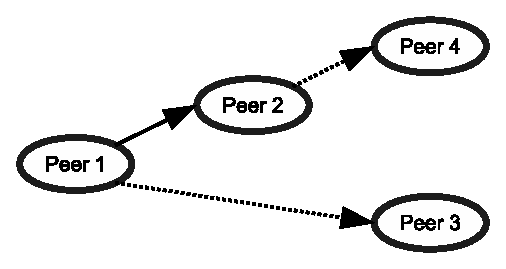
\includegraphics[width=6cm]{logarithmicmodel}
\caption{Logarithmic distribution}
\label{fig:logarithmicmodel}
\end{figure}

The implementation of this model increases the complexity only marginal, but the efficiency is significantly higher. The more peers there are participating the higher is the efficiency. The overhead is also very manageable because during the transfers the idle peers do nothing except waiting. The problem of this model is that never more than 50\% of all peers are uploading in parallel. Also at the beginning only one peer uploads the data set. This means that in the beginning a majority of all peers do not use their upload bandwidth. This model is implemented in the Logarithmic algorithm, which can be found in section \ref{subsubsec:seqlog}.

At the end this model cannot provide the $2 \cdot T_0$ limit we are looking for. To do so this model has to be improved, which is done in the next section \ref{sec:chunkedswarmmodel}.


\section{Model: Chunked-Swarm}
\label{sec:chunkedswarmmodel}
The Chunked-Swarm model is an enhancement of the logarithmic model. It allows multiple uploads in parallel and splits the data set into chunks before transferring it. So peers cannot download the whole data set at once, but have to request each chunk individually instead. Since the size of those chunks is smaller than the size of the whole data set, the peers can help to distribute the data set more quickly. The figure \ref{fig:chunkedswarmmodel} shows 4 peers distributing 3 chunks. At first peer 1 has the data set completely. Peer 2, 3 and 4 each request one chunk in parallel. Those peers will then distribute their chunks among themselves. This means that those peers announce their own chunks to the other peers, which can then request those chunks. It is important to note, that this model is always pull-based. A chunk is only uploaded if a peer explicitly requests it.

\begin{figure}[H]
\centering
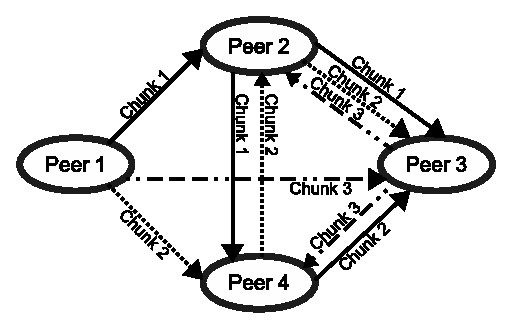
\includegraphics[width=6cm]{chunkedswarmmodel}
\caption{Chunked-Swarm distribution}
\label{fig:chunkedswarmmodel}
\end{figure}

The implementation of this model is not as easy as the logarithmic one, because the efficiency totally depends on the choice of the chunks the peer 2, 3 and 4 request from peer 1. Since this approach is pull-based, the peers do not know what the other peers request. This could lead to chunk duplication which decreases the efficiency considerably. Chunk duplication means that two peers request the same chunk from peer 1 and therefore cannot exchange those chunks afterwards. An implementation of this model has to make strong considerations about this issue. The implementation of this model is described in section \ref{subsubsec:chunkedswarm}. This section also explains the problem of chunk selection in more detail.

To determine the efficiency of this model, it is assumed, that the chunk selection works perfectly, which means that all peers request distinct chunks from peer 1. This also implies that there have to be at least as many chunks as there are peers. Less chunks would also work, but then chunk duplication cannot be prevented.

For simplicity it is also assumed, that there are just as many chunks as there are peers. It this case, it would take $T_0$ seconds to transfer all distinct chunks to all peers, because every peer gets a third of the available bandwidth and also has to download a third of the whole data set. After this, the peers distribute their chunks among themselves, which takes $\frac{2}{3} \cdot T_0$ seconds, as shown in figure \ref{fig:chunkedswarmformula1}.

\begin{figure}[H]
\centering
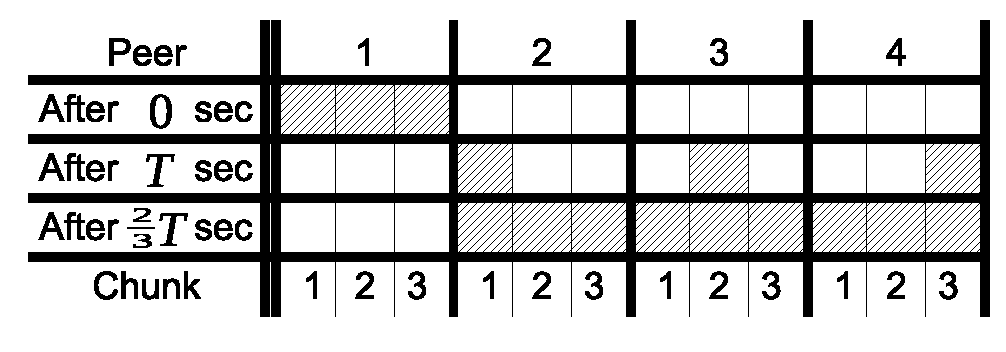
\includegraphics[width=12cm]{chunkedswarmformula1}
\caption{Chunk completion diagramm of the Chunked-Swarm distribution 1}
\label{fig:chunkedswarmformula1}
\end{figure}

This means that after $T = T_0 + \frac{2}{3} \cdot T_0 = \frac{5}{3} \cdot T_0$ seconds every peer has all chunks available. Similiary a variable number of peers need $T(n) = T_0 + \frac{n - 1}{n} \cdot T_0 = \frac{2n - 1}{n} \cdot T_0 = (2 - \frac{1}{n}) \cdot T_0$ seconds. A very nice property of this formula is that the result is always smaller than $2 \cdot T_0$. Without any further optimizations the main objective of this thesis is already fulfilled, as long as the chunk count is equal to or greater than the peer count. But if the chunk count is doubled, the formula gets even better. Figure \ref{fig:chunkedswarmformula2} illustrates this scenario. The efficiency rises because the peers can start to upload their own chunks earlier.

\begin{figure}[H]
\centering
\includegraphics[width=12cm]{chunkedswarmformula2}
\caption{Chunk completion diagramm of the Chunked-Swarm distribution 2}
\label{fig:chunkedswarmformula2}
\end{figure}

After $\frac{1}{2} \cdot T_0$ seconds the peers received the first three distinct chunks from peer 1. At this point the peers can exchange their chunks, which takes $\frac{1}{2} \cdot \frac{2}{3} \cdot T_0$ seconds. After $\frac{5}{6} \cdot T_0$ seconds all peers have the first 50\% of the data set. At $T_0$ seconds the last three distinct chunks arrive which will also be exchanged afterwards. So after $T = T_0 + \frac{1}{2} \cdot \frac{2}{3} \cdot T_0 = \frac{4}{3} \cdot T_0$ seconds all peers have the data set. The general formula is $T(n, c) = T_0 + \frac{n}{c} \cdot \frac{n-1}{n} \cdot T_0 =  T_0 + \frac{n-1}{c} \cdot T_0$, where $c = n \cdot 2^i, i \in \mathbb{N}$ is the chunk count.

Using this relationship the time $T(n, c) = T_0 + \frac{n-1}{c} \cdot T_0$ can almost be minized to $T_0$ if $c >> n$. A major disadvantage is that the chunk count has to be choosen before the transfer can actually happen. Since the efficiency depends on the $\frac{n-1}{c}$ ratio, the maximal number of peers should be determined before. Chapter \ref{sec:streaming} and \ref{ch:futurework} explains in more detail how to use model to implement incremental data set transfers like video or audio streaming.




\cleardoublepage
\chapter{Architecture}
\label{ch:arch}

\begin{figure}[ht]
	\centering
	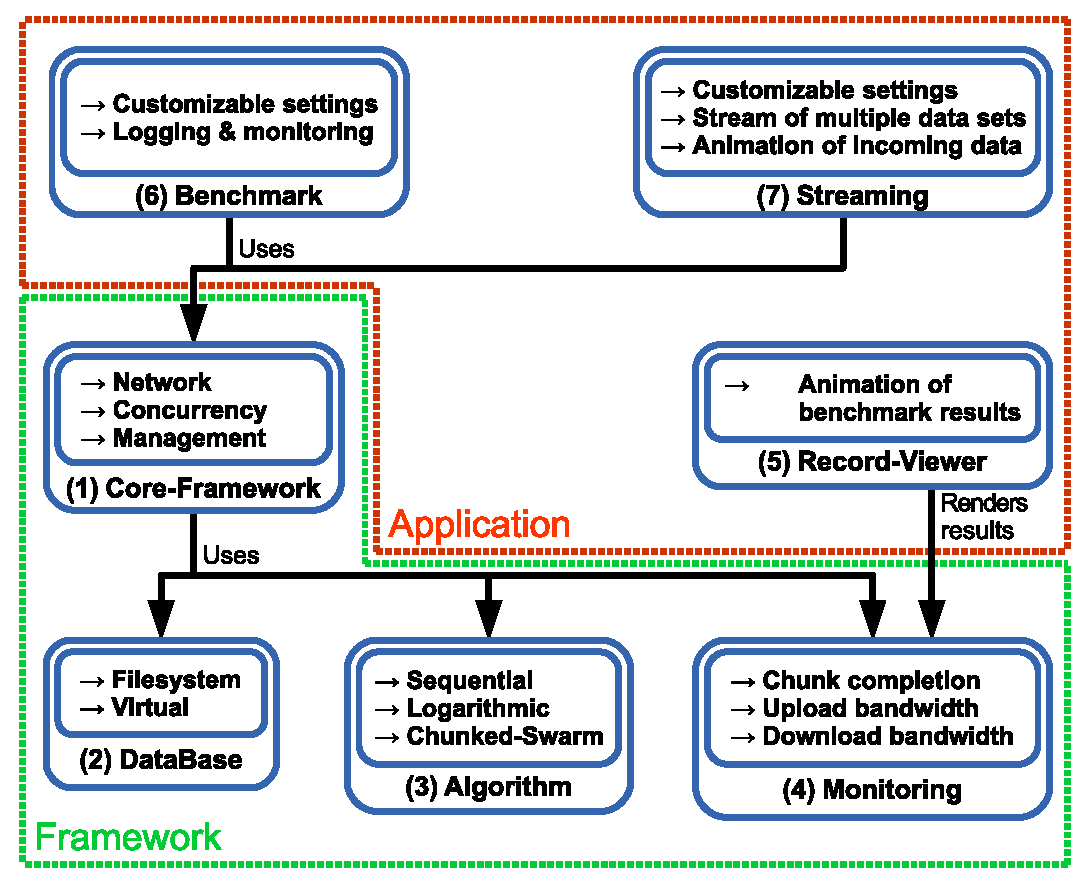
\includegraphics[width=0.9\linewidth]{arch}
	\caption{Software architecture}
	\label{fig:arch}
\end{figure}

This chapter explains the architecture of the software in detail. From the beginning, one of the main goals were to achive high modularity, so individual parts can be enhanced or replaced easily. The software is separated into the framework and the application part, which consists of multiple modules. Figure \ref{fig:arch} shows the architecture. 

The application part depends on the Core-Framework and the Monitoring module. It contains three modules which are Benchmark, Streaming and Record-Viewer. The Benchmark module is the most important application part, because it can help to create, monitor and evaluate different scenarios in terms of performance and efficiency. All measurements were done using this module. The Streaming module is related to future work and demonstrates the possibility for an incremental stream of data sets. The Record-Viewer module can render and animate results taken from the Monitoring module, which belongs to the framework part and thus only depends on it.

The framework part contains the Core-Framework, DataBase, Algorithm and Monitoring module. While the DataBase, Algorithm and Monitoring module can be replaced or even omitted the Core-Framework module is the most important module. It manages network, concurrency and the communication of the three other modules located in the framework part. The DataBase module represents an interface for a generic data storage, which might be the file system or even completely in-memory. The Algorithm module contains the implementations of the concepts presented in chapter \ref{ch:theory}. To implement and test new distribution algorithms only this module has to be modified. The Monitoring module records data like current bandwidth usage and chunk completion, which are important data for evaluating algorithms. This module creates csv files, which can be plotted with tools like gnuplot and a log file, which contains a chronological stream of events occured during the recording and can be rendered using the Record-Viewer module.

In the next two chapters the framework and application modules are explained in detail. The order is bottom-up, which means the Core-Framework module is explained first in section \ref{sec:core} followed by the DataBase, Algorithm and Monitoring module in section \ref{sec:database}, \ref{sec:algorithm} and \ref{sec:monitoring} respectively. The application modules are explained in section \ref{sec:benchmark}, \ref{sec:recordviewer} and \ref{sec:streaming} referring to the Benchmark, Record-Viewer and Streaming module respectively.
\cleardoublepage
\chapter{Framework Modules}
\section{Module: Core-Framework}
\label{sec:core}
\subsection{Network}
The network implementation has the concept of leechers and seeders. A leecher connects to one or more seeders and requests chunks from them. A seeder has multiple leechers connected to it and answers to chunk requests. Every chunk transfer is pull-based, which means it can only be requested by the leecher while every non-chunk transfer like Meta-Data or address announcements is always push-based, which means that a seeder transfers them without being asked to do so. This has the advantage that every leecher knows exactly what a seeder has to offer without asking but only requests the chunks it needs. See section \ref{subsubsec:downloadreq} for more information.

While leechers and seeders are independent of each other it is possible to couple them together. A leecher coupled with a seeder always announces the address of its seeder to any other seeder it is connected with. This concept is explained in more detail in section \ref{subsubsec:autoconnect}.

Both a leecher and a seeder keep a reference to a database instance. A leecher stores downloaded chunks in its database and a seeder uploads chunks from its database. It is possible that both a leecher and a seeder reference the same database instance in which case the seeder is able to upload every downloaded chunk from the leecher. The DataBase module and all related concepts are explained in section \ref{sec:database}.

A leecher and a seeder both are associated with one of the multiple distribution algorithms defined in the Algorithm module. Those algorithms determine the distribution behaviour, which is further described in section \ref{sec:algorithm}.

\subsubsection{Automatic Connect}
\label{subsubsec:autoconnect}
While every leecher has to manually connect to a seeder for the first time, after this a leecher is able to automatically connect to other seeders. This is because every leecher who is coupled with a seeder announces the address of its coupled seeder to all other seeders it is currently connected with. The figure \ref{fig:autoconnect} show this in detail.

\begin{figure}[H]
\centering
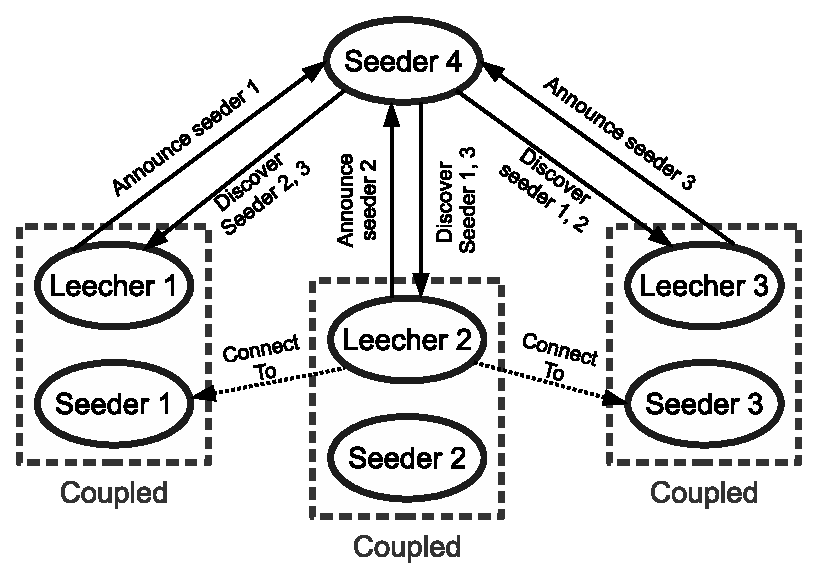
\includegraphics[width=8cm]{autoconnect}
\caption{Seeder Discovery}
\label{fig:autoconnect}
\end{figure}

Here leecher 1, 2 and 3 announce the address of seeder 1, 2 and 3 respectively to seeder 4 which then broadcasts those addresses to all connected leechers. This way the leechers get to know each other and can connect to the remaining seeders. Though in figure \ref{fig:autoconnect} only leecher 2 is illustrated, leecher 1 and 3 connect to the other seeders as well. Of course, this works recursively, so if one of the seeders 1, 2 or 3 already has other leechers connected to it those will also be found. So in the end the topology is just a mesh with $(n-1)^2$ connections where $n$ refers to the total number of peers and every leecher of each peer is connected to every seeder of all other peers. The figure \ref{fig:mesh} shows this from the point of view of leecher 1 from peer 1 assuming there are 7 other peers.

\begin{figure}[H]
\centering
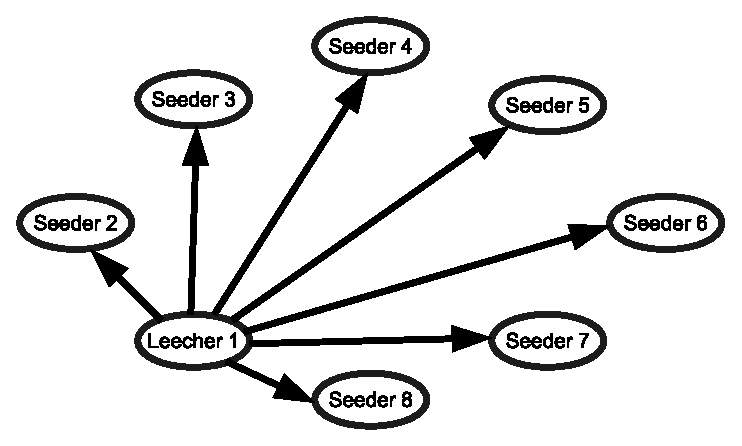
\includegraphics[width=8cm]{mesh}
\caption{Mesh topology}
\label{fig:mesh}
\end{figure}

While this topology is really great in terms of knowledge where every peer knows exactly what data sets the other peers have and thus can request chunks efficiently, it is also quite expensive and would not scale indefinitely. To improve scalability and reduce efficiency the number of connections per leecher can be limited which limits the knowledge of each leecher and thus the ability to make good decisions what to request from whom. This is explained later in section \ref{sec:benchmark} in more detail.

If a leecher loses, for what ever reason, the connection to a seeder the framework is able to reconnect if the seeder is still online. This will be detected by periodic address broadcasts. So if for instance leecher 1 lost the connection to seeder 2 but leecher 1 and 2 are also connected to seeder 3 then seeder 3 will notify leecher 1 that seeder 2 still exists. The figure \ref{fig:reconnect} illustrates this.

\begin{figure}[H]
\centering
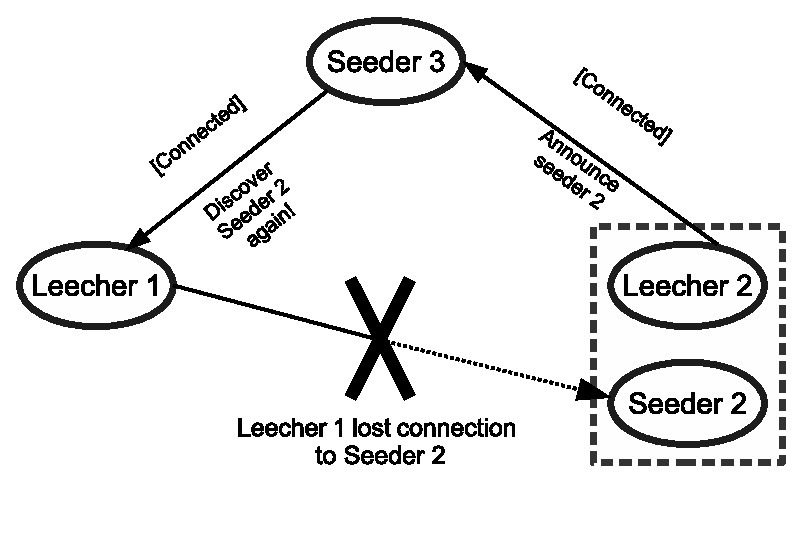
\includegraphics[width=8cm]{reconnect}
\caption{Reconnect}
\label{fig:reconnect}
\end{figure}


\subsubsection{Meta-Data Announcements}
After a leecher connects to a seeder the leecher does not know anything about the seeder. As previously explained in section \ref{subsubsec:autoconnect} the leecher discovers new seeders through the seeders it is currently connected to. The way the leecher gets knowlege about what data sets a seeder offers works a similiar way. A seeder announces to all connected leechers periodically what data sets it has to offer. It basically transfers a list of Meta-Data, which is explained further in section \ref{subsubsec:metadata}, so that every leecher can update its knowledge about the seeder. The list of Meta-Data can be modified before it is announced by the used distribution algorithm to model a specific distribution behaviour, see section \ref{sec:algorithm} for further information.

As an optimization the seeder only transfers new Meta-Data. So if a data set does not change at all, a seeder will never transfer a second announcement of this data set. Another optimization is that while a leecher downloads a chunk from a seeder, the seeder will also not transfer any announcements during this period, which is explained further in the next section \ref{subsubsec:downloadreq}.


\subsubsection{Download Requests}
\label{subsubsec:downloadreq}
After a leecher successfully connected to one or more seeders and already received Meta-Data announcements it can start to request chunks from the seeders. What to request from whom heavily depends on the used distribution algorithm, which is explained in section \ref{sec:algorithm} in more detail. 

Since downloading more than one chunk at a time from a seeder is not faster than downloading them sequentially only one download at a time is allowed which also reduces protocol complexity. Because of that Meta-Data and address announcements are also not transferred during a chunk download because those announcements are then obviously of no interest for the leecher. As soon as the chunk download completes outstanding announcements are bundled and transferred.

A seeder is allowed to decide whether or not a chunk request is valid, which means that depending on the algorithm the seeder can reject a chunk request. If a seeder rejects a chunk request the leecher do not request the same chunk again. The seeder can tell the leecher that a previously rejected chunk request is valid again by reannouncing the specific chunk. This way complex distribution behaviour can easily be implemented.


\subsubsection{Nonblocking I/O}
Network communication is based on sockets. Sockets can either be datagram or stream based. Datagram sockets have no notion of connections and are of no importance for this thesis. Instead the network implementation uses stream sockets. A stream socket is always connected to an other socket. Those two sockets behave like files. If you write data to a socket it is transferred to the other socket and can then be read from it. As with files, socket operations usually block the currently executing thread until the requested data is read or written. This implies that you basically need one thread per socket to handle multiple sockets concurrently. Unfortunately threads are a limited resource and thus this concept does not scale well. 

To improve this situation nonblocking sockets in combination with event-polling were introduced, where you are notified when a socket operation can be executed without blocking. This way you can theoretically serve tens of thousands of sockets in a single thread. Since this thesis concentrates on large-scale this technique is a must-have.

The problem with nonblocking sockets is that it increases the complexity significantly so the network implementation uses a framework to simplify the usage. The framework is called Netty 5 and written in Java. One great thing about Netty is that it totally separates the transport protocol oriented code from the logic oriented one. This way it does not matter which transport protocol you use as long as this protocol is stream based.


\subsubsection{Transport: Local and TCP}
Netty offers a Local (also called In-VM) transport protocol which does not involve network at all. It only works inside a single instance of the JVM and is perfectly suited for simulations or benchmarking. That is because the Local transport does not require you to serialize and deserialize the data which eliminates a huge amount of memory and CPU usage. In normal usage the overhead of serialization is negligible but since the Benchmark module is able to simulate a large number of seeders and leechers, see section \ref{sec:benchmark}, those overheads can start to sum up. The Local transport seems to be the perfect fit for this purpose.

Netty also offers usual transport protocols like TCP. It is used as secondary option for the Benchmark module which is useful if you want to run distributed benchmark on multiple machines since Local transport is limited to a single JVM instance.


\subsubsection{Traffic-Shaping}
To simulate and evaluate network applications you need the ability to control the bandwidth in some way to have comparable network conditions. The problem with bandwidth limitation, which is also called traffic-shaping, is that most times you cannot throttle the writer. The writer can either be writing as fast as possible or not writing at all. So in order to limit the bandwidth you have to start and stop the writer periodically.

If the period is too long the introduced bandwidth peaks can affect the measurements in a negative way but if the period is too short instead, you introduce a lot of overhead. To perfectly limit the bandwidth you would need to use a period which is indefinitely short. So if you want to implement traffic-shaping reliably, you must find the sweet spot between accuracy and minimal overhead. The network implementation uses a period of 250 ms which is good enough because the measurements are done every second. So every measurement contains the average of approximately 4 bandwidth limitation runs.

The complexity increases if multiple writers together are not allowed to exceed a given bandwidth. The main problem is fairness. You do not want that one writer gets 95\% of the bandwidth while the remaining writes get only 5\% together. But at the same time you want that a single writer is able to write at full speed if no other writer is writing. This complex behaviour can be achieved using a Leaky-Bucket algorithm and a Priority-Queue.

The Leaky-Bucket contains tokens, where one token equals one byte. If a writer wants to write a message it tries to remove the tokens needed for the message to transfer. If the bucket does not have enough tokens, the writer takes the remaining tokens and decreases the size of the message it want to write by the number of removed tokens. After this it waits until the bucket gets refilled and repeats the action. Unfortunately this does not fix the fairness problem.

To solve the fairness problem a writer is not allowed to remove tokens from the bucket directly. Instead it inserts the write request into a Priority-Queue. A writer-job constantly polls the head of the queue and tries to process the write request using the Leaky-Bucket. The difference is that after writing the message the writer increases its number of total written bytes. If the writer has more message to write it inserts itself into the queue according to the number of total written bytes compared to other writers. This way the head of the queue always is a write request belonging to a writer which has written least. This way you get good fairness with almost no overhead because the writer-job runs only on demand in a thread pool and quits after all write requests are processed.

\cleardoublepage
\subsection{Concurrency}
With the use of nonblocking sockets it is possible to handle a lot of sockets with only one thread. But this can be further improved because modern CPUs always have multiple cores whose quantity determines the number of threads able to run in parallel. If your CPU has 4 cores and you are using only one thread then you cannot use more than 25\% of your CPU capacity. Because of that Netty uses more than one thread to increase the efficiency. In the next section \ref{subsecsec:eventloop} the utilization of multiple threads is explained in more detail.

\subsubsection{Event-Loop}
\label{subsecsec:eventloop}
Netty has the notion of an Event-Loop. An Event-Loop is always running in its own thread and processes queued events one after the other. Those events are mostly readiness events which say that a given socket is now readable, writable, acceptable or connectable.

To use more than one thread Netty simply spawns more Event-Loops, typically just as many as there are CPU cores. New sockets will then be distributed evenly among all running Event-Loops. Even if the Event-Loops get unbalanced Netty tries to rearrange the sockets to become balanced again.

Those Event-Loops can then run theoretically in parallel, because the underlying operating system distributes busy threads equally among all available cores. But using more than one thread is only the tip of the iceberg, multiple threads introduce a whole new category of problems and considerations which have to be taken into account. The next section \ref{subsecsec:lockfree} discusses this a bit more in depth.


\subsubsection{Lock-Free-Progamming}
\label{subsecsec:lockfree}
The main problem when using multiple threads is the question of how those threads interact which each other. If two threads access the same variable without any protection the resulting behaviour is not always defined and can lead to untraceable bugs. The unprotected access of variables is also called a critical-section.

A simple solution is to protect those sections with a mutex lock which simply forbids that more than one thread is entering the critical-section at a time but this decreases efficiency and increase thread context switching which is expensive. One solution is to use lock-free algorithms which exploit certain guarantees made by the Java Memory-Model. To explain those concepts in detail would arguably exceed the boundries of this thesis but it should be noted that the implemention heavily uses those algorithms.

The reason why those concepts were considered is that inter-thread-communication is a key design choice in order to simplify the architecture of the implementation. For instance a leecher can be connected to a lot of seeders receiving a lot of Meta-Data and address announcements. In order to effectively request downloads from the seeders the leecher has to collect the information from all connections which may run in different threads and thus are not protected by default against concurrent access. Since this collection is a very common task it should be optimized as well. Using CAS and volatile operations the overhead can be reduced drastically. In normal situations those overheads can be ignored but if you simulate 1.000 peers on 16 cores this means that you actually have 1.000.000 connections each gathering Meta-Data across 16 threads. If every collection of Meta-Data would stop the world by using a mutex the overhead would start to be noticeable. Those impacts are hard to measure or quantify, though. But in principle the lock-free approach scales better.

\cleardoublepage
\section{Module: DataBase}
\label{sec:database}
The DataBase module represents a generic interface for storing binary data in any kind of storage. While the Core-Framework transfers data between peers the data has to be read from and written to some kind of database. The data managed by the database is not just plain data but chunked data instead. Because of that a database stores so called data sets which consist of multiple chunks. 

The database has the responsibility to verify stored chunks in terms of consistency and validation. But to do so the storage has to know about the structure of the data set. Because of that the Meta-Data which describes a given data set is stored together with the data set as key-value pairs. The next section \ref{subsubsec:metadata} describes the Meta-Data format in more detail.

\subsubsection{Meta-Data}
\label{subsubsec:metadata}
The Meta-Data contains information about a given data set. Those information are transferred between seeders and leechers to describe what data sets are avaiable for download. Those information are:
\begin{itemize} 
\itemsep0pt
\item Name
\item Description
\item ID
\item Size
\item Chunks
\item Hash
\item ChunkHashes
\end{itemize}
The Name and Description fields are used for human-related tasks. The ID has to be globally unique and is used for streaming purposes which will be explained later in section \ref{sec:streaming}. The Size field determines the total size of the data set including all chunks which leads to the next field. The Chunks field is a bit set which simply stores one or zero bits for existing or missing chunks respectively. The length of the bit set determins the number of chunks a data set has. The Hash field contains a checksum generated by a strong hash algorithm like SHA from the whole data set. The ChunkHashes field does the same but for each chunk individually. This way the storage can verify single chunks as well as the data set in total. The reason why there is an extra Hash field for the whole data set is to reduce the chance of hash collision. Two data sets are equal if all of their fields are also equal.

\subsubsection{Backends: In-Memory and Filesystem}
The In-Memory backend stores data sets in main memory and is not persistent. It is a useful backend for situations where you generate or consume data sets on the fly like video streaming or test scenarios.

In case of streaming you can simply add fake data set sources which loads chunks from a live camera or similiar devices.

The Benchmark modules uses this backend to reduce overhead introduced by the filesystem. This backend almost has no overhead other than memory usage.

Related to future work is the filesystem backend which implements a persistent database based on a filesystem. The filesystem can also be virtual like a ZIP file. This backend is more rigid but also very important for file-sharing applications.

\section{Module: Algorithm}
\label{sec:algorithm}

\section{Module: Monitoring}
\label{sec:monitoring}


\cleardoublepage
\chapter{Application Modules}
\label{ch:app}

\section{Module: Benchmark}
\label{sec:benchmark}

The Benchmark module 

\section{Module: Record-Viewer}
\label{sec:recordviewer}

\section{Module: Streaming}
\label{sec:streaming}


\cleardoublepage
%!TEX root = bachelor.tex

\chapter{Evaluation}
\label{evaluation}

\pagebreak
\begin{figure}[ht]
	\begin{center}
		\subfigure[Completion\label{fig:s1:completion}]{
	 		\includegraphics[width=0.5\textwidth]{plots/scenario_1_default/plots/GeneratedMeanChunkCompletion.csv}
	 	}~ % No whitespace here!
	 	\subfigure[Leecher Download Bandwidth\label{fig:s1:download}]{
	 		\includegraphics[width=0.5\textwidth]{plots/scenario_1_default/plots/GeneratedMeanCurrentDownloadBandwidth.csv}
	 	}

		\subfigure[Seeder Upload Bandwidth\label{fig:s1:upload}]{
	 		\includegraphics[width=0.5\textwidth]{plots/scenario_1_default/plots/GeneratedMeanCurrentUploadBandwidth.csv}
	 	}~ % No whitespace here!
	 	\subfigure[Super Seeder Upload Bandwidth\label{fig:s1:ssupload}]{
	 		\includegraphics[width=0.5\textwidth]{plots/scenario_1_default/plots/GeneratedMeanCurrentSuperSeederUploadBandwidth.csv}
	 	}

		\subfigure[Completion\label{fig:s1:scompletion}]{
	 		\includegraphics[width=0.5\textwidth]{plots/scenario_1_default/plots/GeneratedMeanSortedChunkCompletion.csv}
	 	}~ % No whitespace here!
		\caption{Scenario 1 Default}
		\label{fig:s1}
	\end{center}
\end{figure}



\pagebreak
\begin{figure}[ht]
	\begin{center}
		\subfigure[Completion\label{fig:s2:completion}]{
	 		\includegraphics[width=0.5\textwidth]{plots/scenario_2_seq/plots/GeneratedMeanChunkCompletion.csv}
	 	}~ % No whitespace here!
	 	\subfigure[Leecher Download Bandwidth\label{fig:s2:download}]{
	 		\includegraphics[width=0.5\textwidth]{plots/scenario_2_seq/plots/GeneratedMeanCurrentDownloadBandwidth.csv}
	 	}
	
	 	\subfigure[Super Seeder Upload Bandwidth\label{fig:s2:ssupload}]{
	 		\includegraphics[width=0.5\textwidth]{plots/scenario_2_seq/plots/GeneratedMeanCurrentSuperSeederUploadBandwidth.csv}
	 	}~ % No whitespace here!
		\subfigure[Completion\label{fig:s2:scompletion}]{
	 		\includegraphics[width=0.5\textwidth]{plots/scenario_2_seq/plots/GeneratedMeanSortedChunkCompletion.csv}
	 	}~ % No whitespace here!
		\caption{Scenario 2 Sequential}
		\label{fig:s2}
	\end{center}
\end{figure}



\pagebreak
\begin{figure}[ht]
	\begin{center}
		\subfigure[Completion\label{fig:s3:completion}]{
	 		\includegraphics[width=0.5\textwidth]{plots/scenario_3_log/plots/GeneratedMeanChunkCompletion.csv}
	 	}~ % No whitespace here!
	 	\subfigure[Leecher Download Bandwidth\label{fig:s3:download}]{
	 		\includegraphics[width=0.5\textwidth]{plots/scenario_3_log/plots/GeneratedMeanCurrentDownloadBandwidth.csv}
	 	}

		\subfigure[Seeder Upload Bandwidth\label{fig:s3:upload}]{
	 		\includegraphics[width=0.5\textwidth]{plots/scenario_3_log/plots/GeneratedMeanCurrentUploadBandwidth.csv}
	 	}~ % No whitespace here!
	 	\subfigure[Super Seeder Upload Bandwidth\label{fig:s3:ssupload}]{
	 		\includegraphics[width=0.5\textwidth]{plots/scenario_3_log/plots/GeneratedMeanCurrentSuperSeederUploadBandwidth.csv}
	 	}

		\subfigure[Completion\label{fig:s3:scompletion}]{
	 		\includegraphics[width=0.5\textwidth]{plots/scenario_3_log/plots/GeneratedMeanSortedChunkCompletion.csv}
	 	}~ % No whitespace here!
		\caption{Scenario 3 Logarithmic}
		\label{fig:s3}
	\end{center}
\end{figure}



\pagebreak
\begin{figure}[ht]
	\begin{center}
		\subfigure[Completion\label{fig:s4:completion}]{
	 		\includegraphics[width=0.5\textwidth]{plots/scenario_4_peer_count_128/plots/GeneratedMeanChunkCompletion.csv}
	 	}~ % No whitespace here!
	 	\subfigure[Leecher Download Bandwidth\label{fig:s4:download}]{
	 		\includegraphics[width=0.5\textwidth]{plots/scenario_4_peer_count_128/plots/GeneratedMeanCurrentDownloadBandwidth.csv}
	 	}

		\subfigure[Seeder Upload Bandwidth\label{fig:s4:upload}]{
	 		\includegraphics[width=0.5\textwidth]{plots/scenario_4_peer_count_128/plots/GeneratedMeanCurrentUploadBandwidth.csv}
	 	}~ % No whitespace here!
	 	\subfigure[Super Seeder Upload Bandwidth\label{fig:s4:ssupload}]{
	 		\includegraphics[width=0.5\textwidth]{plots/scenario_4_peer_count_128/plots/GeneratedMeanCurrentSuperSeederUploadBandwidth.csv}
	 	}

		\subfigure[Completion\label{fig:s4:scompletion}]{
	 		\includegraphics[width=0.5\textwidth]{plots/scenario_4_peer_count_128/plots/GeneratedMeanSortedChunkCompletion.csv}
	 	}~ % No whitespace here!
		\caption{Scenario 4 Peer Count 128}
		\label{fig:s4}
	\end{center}
\end{figure}



\pagebreak
\begin{figure}[ht]
	\begin{center}
		\subfigure[Completion\label{fig:s5:completion}]{
	 		\includegraphics[width=0.5\textwidth]{plots/scenario_5_meta_data_0/plots/GeneratedMeanChunkCompletion.csv}
	 	}~ % No whitespace here!
	 	\subfigure[Leecher Download Bandwidth\label{fig:s5:download}]{
	 		\includegraphics[width=0.5\textwidth]{plots/scenario_5_meta_data_0/plots/GeneratedMeanCurrentDownloadBandwidth.csv}
	 	}

		\subfigure[Seeder Upload Bandwidth\label{fig:s5:upload}]{
	 		\includegraphics[width=0.5\textwidth]{plots/scenario_5_meta_data_0/plots/GeneratedMeanCurrentUploadBandwidth.csv}
	 	}~ % No whitespace here!
	 	\subfigure[Super Seeder Upload Bandwidth\label{fig:s5:ssupload}]{
	 		\includegraphics[width=0.5\textwidth]{plots/scenario_5_meta_data_0/plots/GeneratedMeanCurrentSuperSeederUploadBandwidth.csv}
	 	}

		\subfigure[Completion\label{fig:s5:scompletion}]{
	 		\includegraphics[width=0.5\textwidth]{plots/scenario_5_meta_data_0/plots/GeneratedMeanSortedChunkCompletion.csv}
	 	}~ % No whitespace here!
		\caption{Scenario 5 Meta Data 0}
		\label{fig:s5}
	\end{center}
\end{figure}



\pagebreak
\begin{figure}[ht]
	\begin{center}
		\subfigure[Completion\label{fig:s6:completion}]{
	 		\includegraphics[width=0.5\textwidth]{plots/scenario_6_parts_20/plots/GeneratedMeanChunkCompletion.csv}
	 	}~ % No whitespace here!
	 	\subfigure[Leecher Download Bandwidth\label{fig:s6:download}]{
	 		\includegraphics[width=0.5\textwidth]{plots/scenario_6_parts_20/plots/GeneratedMeanCurrentDownloadBandwidth.csv}
	 	}

		\subfigure[Seeder Upload Bandwidth\label{fig:s6:upload}]{
	 		\includegraphics[width=0.5\textwidth]{plots/scenario_6_parts_20/plots/GeneratedMeanCurrentUploadBandwidth.csv}
	 	}~ % No whitespace here!
	 	\subfigure[Super Seeder Upload Bandwidth\label{fig:s6:ssupload}]{
	 		\includegraphics[width=0.5\textwidth]{plots/scenario_6_parts_20/plots/GeneratedMeanCurrentSuperSeederUploadBandwidth.csv}
	 	}

		\subfigure[Completion\label{fig:s6:scompletion}]{
	 		\includegraphics[width=0.5\textwidth]{plots/scenario_6_parts_20/plots/GeneratedMeanSortedChunkCompletion.csv}
	 	}~ % No whitespace here!
		\caption{Scenario 6 Parts 20}
		\label{fig:s6}
	\end{center}
\end{figure}



\pagebreak
\begin{figure}[ht]
	\begin{center}
		\subfigure[Completion\label{fig:s7:completion}]{
	 		\includegraphics[width=0.5\textwidth]{plots/scenario_7_chunk_count_fac_1/plots/GeneratedMeanChunkCompletion.csv}
	 	}~ % No whitespace here!
	 	\subfigure[Leecher Download Bandwidth\label{fig:s7:download}]{
	 		\includegraphics[width=0.5\textwidth]{plots/scenario_7_chunk_count_fac_1/plots/GeneratedMeanCurrentDownloadBandwidth.csv}
	 	}

		\subfigure[Seeder Upload Bandwidth\label{fig:s7:upload}]{
	 		\includegraphics[width=0.5\textwidth]{plots/scenario_7_chunk_count_fac_1/plots/GeneratedMeanCurrentUploadBandwidth.csv}
	 	}~ % No whitespace here!
	 	\subfigure[Super Seeder Upload Bandwidth\label{fig:s7:ssupload}]{
	 		\includegraphics[width=0.5\textwidth]{plots/scenario_7_chunk_count_fac_1/plots/GeneratedMeanCurrentSuperSeederUploadBandwidth.csv}
	 	}

		\subfigure[Completion\label{fig:s7:scompletion}]{
	 		\includegraphics[width=0.5\textwidth]{plots/scenario_7_chunk_count_fac_1/plots/GeneratedMeanSortedChunkCompletion.csv}
	 	}~ % No whitespace here!
		\caption{Scenario 7 Chunk Count Factor 1}
		\label{fig:s7}
	\end{center}
\end{figure}



\pagebreak
\begin{figure}[ht]
	\begin{center}
		\subfigure[Completion\label{fig:s8:completion}]{
	 		\includegraphics[width=0.5\textwidth]{plots/scenario_8_peer_count_32/plots/GeneratedMeanChunkCompletion.csv}
	 	}~ % No whitespace here!
	 	\subfigure[Leecher Download Bandwidth\label{fig:s8:download}]{
	 		\includegraphics[width=0.5\textwidth]{plots/scenario_8_peer_count_32/plots/GeneratedMeanCurrentDownloadBandwidth.csv}
	 	}

		\subfigure[Seeder Upload Bandwidth\label{fig:s8:upload}]{
	 		\includegraphics[width=0.5\textwidth]{plots/scenario_8_peer_count_32/plots/GeneratedMeanCurrentUploadBandwidth.csv}
	 	}~ % No whitespace here!
	 	\subfigure[Super Seeder Upload Bandwidth\label{fig:s8:ssupload}]{
	 		\includegraphics[width=0.5\textwidth]{plots/scenario_8_peer_count_32/plots/GeneratedMeanCurrentSuperSeederUploadBandwidth.csv}
	 	}

		\subfigure[Completion\label{fig:s8:scompletion}]{
	 		\includegraphics[width=0.5\textwidth]{plots/scenario_8_peer_count_32/plots/GeneratedMeanSortedChunkCompletion.csv}
	 	}~ % No whitespace here!
		\caption{Scenario 8 Peer Count 32}
		\label{fig:s8}
	\end{center}
\end{figure}



\pagebreak
\begin{figure}[ht]
	\begin{center}
		\subfigure[Completion\label{fig:s9:completion}]{
	 		\includegraphics[width=0.5\textwidth]{plots/scenario_9_parts_10/plots/GeneratedMeanChunkCompletion.csv}
	 	}~ % No whitespace here!
	 	\subfigure[Leecher Download Bandwidth\label{fig:s9:download}]{
	 		\includegraphics[width=0.5\textwidth]{plots/scenario_9_parts_10/plots/GeneratedMeanCurrentDownloadBandwidth.csv}
	 	}

		\subfigure[Seeder Upload Bandwidth\label{fig:s9:upload}]{
	 		\includegraphics[width=0.5\textwidth]{plots/scenario_9_parts_10/plots/GeneratedMeanCurrentUploadBandwidth.csv}
	 	}~ % No whitespace here!
	 	\subfigure[Super Seeder Upload Bandwidth\label{fig:s9:ssupload}]{
	 		\includegraphics[width=0.5\textwidth]{plots/scenario_9_parts_10/plots/GeneratedMeanCurrentSuperSeederUploadBandwidth.csv}
	 	}

		\subfigure[Completion\label{fig:s9:scompletion}]{
	 		\includegraphics[width=0.5\textwidth]{plots/scenario_9_parts_10/plots/GeneratedMeanSortedChunkCompletion.csv}
	 	}~ % No whitespace here!
		\caption{Scenario 9 Parts 10}
		\label{fig:s9}
	\end{center}
\end{figure}



\pagebreak
\begin{figure}[ht]
	\begin{center}
		\subfigure[Completion\label{fig:s10:completion}]{
	 		\includegraphics[width=0.5\textwidth]{plots/scenario_10_meta_data_10/plots/GeneratedMeanChunkCompletion.csv}
	 	}~ % No whitespace here!
	 	\subfigure[Leecher Download Bandwidth\label{fig:s10:download}]{
	 		\includegraphics[width=0.5\textwidth]{plots/scenario_10_meta_data_10/plots/GeneratedMeanCurrentDownloadBandwidth.csv}
	 	}

		\subfigure[Seeder Upload Bandwidth\label{fig:s10:upload}]{
	 		\includegraphics[width=0.5\textwidth]{plots/scenario_10_meta_data_10/plots/GeneratedMeanCurrentUploadBandwidth.csv}
	 	}~ % No whitespace here!
	 	\subfigure[Super Seeder Upload Bandwidth\label{fig:s10:ssupload}]{
	 		\includegraphics[width=0.5\textwidth]{plots/scenario_10_meta_data_10/plots/GeneratedMeanCurrentSuperSeederUploadBandwidth.csv}
	 	}

		\subfigure[Completion\label{fig:s10:scompletion}]{
	 		\includegraphics[width=0.5\textwidth]{plots/scenario_10_meta_data_10/plots/GeneratedMeanSortedChunkCompletion.csv}
	 	}~ % No whitespace here!
		\caption{Scenario 10 Meta Data 10}
		\label{fig:s10}
	\end{center}
\end{figure}



\pagebreak
\begin{figure}[ht]
	\begin{center}
		\subfigure[Completion\label{fig:s11:completion}]{
	 		\includegraphics[width=0.5\textwidth]{plots/scenario_11_peer_count_192_v2/plots/GeneratedMeanChunkCompletion.csv}
	 	}~ % No whitespace here!
	 	\subfigure[Leecher Download Bandwidth\label{fig:s11:download}]{
	 		\includegraphics[width=0.5\textwidth]{plots/scenario_11_peer_count_192_v2/plots/GeneratedMeanCurrentDownloadBandwidth.csv}
	 	}

		\subfigure[Seeder Upload Bandwidth\label{fig:s11:upload}]{
	 		\includegraphics[width=0.5\textwidth]{plots/scenario_11_peer_count_192_v2/plots/GeneratedMeanCurrentUploadBandwidth.csv}
	 	}~ % No whitespace here!
	 	\subfigure[Super Seeder Upload Bandwidth\label{fig:s11:ssupload}]{
	 		\includegraphics[width=0.5\textwidth]{plots/scenario_11_peer_count_192_v2/plots/GeneratedMeanCurrentSuperSeederUploadBandwidth.csv}
	 	}

		\subfigure[Completion\label{fig:s11:scompletion}]{
	 		\includegraphics[width=0.5\textwidth]{plots/scenario_11_peer_count_192_v2/plots/GeneratedMeanSortedChunkCompletion.csv}
	 	}~ % No whitespace here!
		\caption{Scenario 11 Peer Count 192}
		\label{fig:s11}
	\end{center}
\end{figure}



\pagebreak
\begin{figure}[ht]
	\begin{center}
		\subfigure[Completion\label{fig:s12:completion}]{
	 		\includegraphics[width=0.5\textwidth]{plots/scenario_12_peer_count_256/plots/GeneratedMeanChunkCompletion.csv}
	 	}~ % No whitespace here!
	 	\subfigure[Leecher Download Bandwidth\label{fig:s12:download}]{
	 		\includegraphics[width=0.5\textwidth]{plots/scenario_12_peer_count_256/plots/GeneratedMeanCurrentDownloadBandwidth.csv}
	 	}

		\subfigure[Seeder Upload Bandwidth\label{fig:s12:upload}]{
	 		\includegraphics[width=0.5\textwidth]{plots/scenario_12_peer_count_256/plots/GeneratedMeanCurrentUploadBandwidth.csv}
	 	}~ % No whitespace here!
	 	\subfigure[Super Seeder Upload Bandwidth\label{fig:s12:ssupload}]{
	 		\includegraphics[width=0.5\textwidth]{plots/scenario_12_peer_count_256/plots/GeneratedMeanCurrentSuperSeederUploadBandwidth.csv}
	 	}

		\subfigure[Completion\label{fig:s12:scompletion}]{
	 		\includegraphics[width=0.5\textwidth]{plots/scenario_12_peer_count_256/plots/GeneratedMeanSortedChunkCompletion.csv}
	 	}~ % No whitespace here!
		\caption{Scenario 12 Peer Count 256}
		\label{fig:s12}
	\end{center}
\end{figure}



\pagebreak
\begin{figure}[ht]
	\begin{center}
		\subfigure[Completion\label{fig:s15:completion}]{
	 		\includegraphics[width=0.5\textwidth]{plots/scenario_15_chunk_count_fac_4/plots/GeneratedMeanChunkCompletion.csv}
	 	}~ % No whitespace here!
	 	\subfigure[Leecher Download Bandwidth\label{fig:s15:download}]{
	 		\includegraphics[width=0.5\textwidth]{plots/scenario_15_chunk_count_fac_4/plots/GeneratedMeanCurrentDownloadBandwidth.csv}
	 	}

		\subfigure[Seeder Upload Bandwidth\label{fig:s15:upload}]{
	 		\includegraphics[width=0.5\textwidth]{plots/scenario_15_chunk_count_fac_4/plots/GeneratedMeanCurrentUploadBandwidth.csv}
	 	}~ % No whitespace here!
	 	\subfigure[Super Seeder Upload Bandwidth\label{fig:s15:ssupload}]{
	 		\includegraphics[width=0.5\textwidth]{plots/scenario_15_chunk_count_fac_4/plots/GeneratedMeanCurrentSuperSeederUploadBandwidth.csv}
	 	}

		\subfigure[Completion\label{fig:s15:scompletion}]{
	 		\includegraphics[width=0.5\textwidth]{plots/scenario_15_chunk_count_fac_4/plots/GeneratedMeanSortedChunkCompletion.csv}
	 	}~ % No whitespace here!
		\caption{Scenario 15 Chunk Count Factor 4}
		\label{fig:s15}
	\end{center}
\end{figure}



\pagebreak
\begin{figure}[ht]
	\begin{center}
		\subfigure[Completion\label{fig:s16:completion}]{
	 		\includegraphics[width=0.5\textwidth]{plots/scenario_16_chunk_count_fac_8/plots/GeneratedMeanChunkCompletion.csv}
	 	}~ % No whitespace here!
	 	\subfigure[Leecher Download Bandwidth\label{fig:s16:download}]{
	 		\includegraphics[width=0.5\textwidth]{plots/scenario_16_chunk_count_fac_8/plots/GeneratedMeanCurrentDownloadBandwidth.csv}
	 	}

		\subfigure[Seeder Upload Bandwidth\label{fig:s16:upload}]{
	 		\includegraphics[width=0.5\textwidth]{plots/scenario_16_chunk_count_fac_8/plots/GeneratedMeanCurrentUploadBandwidth.csv}
	 	}~ % No whitespace here!
	 	\subfigure[Super Seeder Upload Bandwidth\label{fig:s16:ssupload}]{
	 		\includegraphics[width=0.5\textwidth]{plots/scenario_16_chunk_count_fac_8/plots/GeneratedMeanCurrentSuperSeederUploadBandwidth.csv}
	 	}

		\subfigure[Completion\label{fig:s16:scompletion}]{
	 		\includegraphics[width=0.5\textwidth]{plots/scenario_16_chunk_count_fac_8/plots/GeneratedMeanSortedChunkCompletion.csv}
	 	}~ % No whitespace here!
		\caption{Scenario 16 Chunk Count Factor 8}
		\label{fig:s16}
	\end{center}
\end{figure}



\pagebreak
\begin{figure}[ht]
	\begin{center}
		\subfigure[Completion\label{fig:s17:completion}]{
	 		\includegraphics[width=0.5\textwidth]{plots/scenario_17_chunk_count_fac_16/plots/GeneratedMeanChunkCompletion.csv}
	 	}~ % No whitespace here!
	 	\subfigure[Leecher Download Bandwidth\label{fig:s17:download}]{
	 		\includegraphics[width=0.5\textwidth]{plots/scenario_17_chunk_count_fac_16/plots/GeneratedMeanCurrentDownloadBandwidth.csv}
	 	}

		\subfigure[Seeder Upload Bandwidth\label{fig:s17:upload}]{
	 		\includegraphics[width=0.5\textwidth]{plots/scenario_17_chunk_count_fac_16/plots/GeneratedMeanCurrentUploadBandwidth.csv}
	 	}~ % No whitespace here!
	 	\subfigure[Super Seeder Upload Bandwidth\label{fig:s17:ssupload}]{
	 		\includegraphics[width=0.5\textwidth]{plots/scenario_17_chunk_count_fac_16/plots/GeneratedMeanCurrentSuperSeederUploadBandwidth.csv}
	 	}

		\subfigure[Completion\label{fig:s17:scompletion}]{
	 		\includegraphics[width=0.5\textwidth]{plots/scenario_17_chunk_count_fac_16/plots/GeneratedMeanSortedChunkCompletion.csv}
	 	}~ % No whitespace here!
		\caption{Scenario 17 Chunk Count Factor 16}
		\label{fig:s17}
	\end{center}
\end{figure}

























\cleardoublepage
\chapter{Future work}
\label{ch:futurework}

%%%%%%%%%%%%%%%%%%%%%%%%%%%%%%%%%%%%%%%%%%%%%%
%%    End of the main document              %%
%%%%%%%%%%%%%%%%%%%%%%%%%%%%%%%%%%%%%%%%%%%%%%

\backmatter

\bibliographystyle{alphadin} %% german output

\bibliography{bibtex-references}

% \printindex

\include{bachelor-declaration}

\cleardoublepage

%!TEX root = bachelor.tex

\chapter*{}
\thispagestyle{empty}

\begin{center}
  \vspace{-3cm}
  \fbox{\parbox[c][12cm][c]{12cm}{\centering Please add here\\[1cm] the DVD holding sheet}}
\end{center}

\vfill

\textbf{This DVD contains:}
\begin{itemize}
 \item A \emph{pdf} Version of this bachelor thesis
 \item All \LaTeX\:and graphic files that have been used, as well as the corresponding scripts
 \item The source code of the software that was created during the bachelor thesis 
 \item The measurement data that was created during the evaluation
\end{itemize}


\end{document}

